\documentclass{article}
\usepackage[utf8]{inputenc}
\usepackage[UTF8]{ctex}
\usepackage{amsthm}
\usepackage{amsmath}
\usepackage{amssymb}
\usepackage{graphicx}
\usepackage{hyperref}
\usepackage[table]{xcolor}
\usepackage{fancyhdr}
\usepackage{lastpage}
\usepackage{pythonhighlight}
\usepackage{subfigure}
\usepackage{fancyhdr}
\usepackage[superscript]{cite}
\usepackage{geometry}
\usepackage{appendix}
\usepackage{listings}
\usepackage[framed,numbered,autolinebreaks,useliterate]{mcode}



\geometry{left=4cm,right=4cm,top=1.5cm,bottom=1.5cm}
\begin{document}
\title{木星磁场的建模与计算}
\author{薛昊天 518021910506}
\date{\small{上海交通大学 电子信息与电气工程学院}}
\maketitle
\begin{abstract}
   木星是太阳系最大的行星,它拥有太阳系最强的行星磁场。木星磁场是木星探测的基本环境之一,因此对木星磁场的建模十分有意义。本文通过借鉴国际地磁场$^{[1]}$的建模计算过程,在木星上类比计算出磁场强度,并对结果进行比较,分析和讨论。\\
  \textbf{关键词:木星,磁场,建模}
  
\end{abstract}




\section{建模过程}
 \subsection{基本假设}
   在本文中,我们假设木星是一个规则球体,半径为$R_J$,参考系使用 Right-handed System III
   (S3RH), 如图1:在这一参考系下,木星表面一个点的经度$\lambda_{RH}$随着自传而减小。
   同时我们假设木星内部的磁场是由恒定电场产生的稳恒磁场,是一个有势无旋场。
   
\begin{figure}
    \centering
    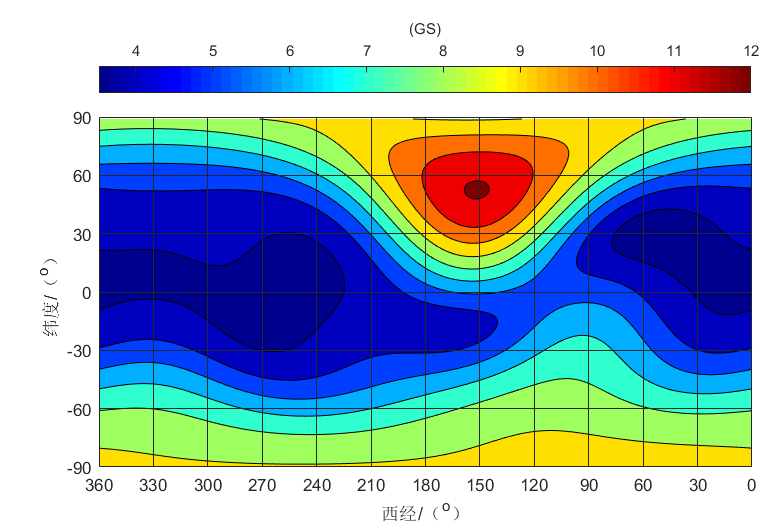
\includegraphics[scale=0.25]{./figure/model.pdf}
    \caption{S3RH木星坐标系}
    \label{fig:my_label}
\end{figure}   

   \subsection{公式}
   首先在麦克斯韦方程组中,在稳恒场中有:
   
   \begin{equation} 
       \nabla \times E = -\frac{\partial{B}}{\partial{t}}=0 
   \end{equation}

   而根据假设的电场条件,有 $E=-\nabla{\varphi}$。在S3RH参考系下,有$\varphi=U(r,\theta,\lambda)$,代入式(1)有:
   
   \begin{equation} 
       \nabla^{2}\varphi=\nabla^{2}U(r,\theta,\lambda)=0
   \end{equation}
   这是一个球坐标下的拉普拉斯方程,表达式可以求出是$^{[2]}$:

    \begin{equation}
        \frac{1}{r^{2}}\frac{\partial}{\partial{r}}(r^2\frac{\partial{U}}{\partial{r}})+\frac{1}{r^2sin\theta}\frac{\partial}{\partial\theta}(sin\theta\frac{\partial{U}}{\partial\theta}) + \frac{1}{r^2sin^2\theta}\frac{\partial^{2}U}{\partial{\lambda}^2}=0
   \end{equation}
   


利用多次的分离变量和边界条件我们就可以求解出木星表面磁场的表达式(详细计算过程见附录A):
\begin{equation}
    U_i(r, \theta,\lambda)=R\sum_{n=1}^{\infty}\sum_{m=0}^{n}(\frac{R}{r})^{n+1}\times(g_{n}^{m}cos(m\lambda)+h_{n}^{m}sin(m\lambda))P^{m}_{n}(cos\theta)
\end{equation}
其中半标准化缔合勒让德函数的一阶导数为:
\begin{equation}
    \frac{dP^{m}_{n}(cos\theta)}{d\theta} = -sin^{m+1}\theta\cdot{P^{m+1}_{n}(cos\theta)}+
    msin^{m-1}\theta{cos}\theta\cdot{P^{m}_{n}(cos\theta)}
\end{equation}

在公式(4)中:r是待测点的径向距离;$\theta$是S3RH中的余纬度,$\lambda$是东经度;$g_n^m,h_n^m$是球谐系数,$P_n^m(x)$是n阶m次的施密特半标准化缔合勒让德函数。所以有对其求梯度可得磁场在三个方向上的分量:

%\includegraphics[scale=1.2]{./figure/ans.PNG}

\begin{equation}
  \left\{
    \begin{array}{l}\vspace{1ex} 
            B_{\theta}=-\frac{\partial{U}}{r\partial\theta}= -R\sum_{n=1}^{\infty}\sum_{m=0}^{n}(\frac{R}{r})^{n+1}\times(g_{n}^{m}cos(m\lambda)+h_{n}^{m}sin(m\lambda))\frac{\partial{P^{m}_{n}}(cos\theta)}{\partial\theta}\\ \vspace{1ex} 
            B_{\lambda}=-\frac{\partial\varphi_i}{rsin\theta\partial\lambda}=R\sum_{n=1}^{\infty}\sum_{m=0}^{n}(\frac{R}{r})^{n+1}\times(g_{n}^{m}cos(m\lambda)-h_{n}^{m}sin(m\lambda))P^{m}_{n}(cos\theta) \\ \vspace{1ex} 
            B_r = -\frac{\partial\varphi_i}{\partial{r}}=R\sum_{n=1}^{\infty}\sum_{m=0}^{n}(n+1)(\frac{R}{r})^{n+1}\times(g_{n}^{m}cos(m\lambda)+h_{n}^{m}sin(m\lambda))P^{m}_{n}(cos\theta)
            
        \end{array}
\right.
\end{equation}


公式(6)也是本文中计算的主要依据,需要注意的是公式里面的$g_n^m,h_n^m$到目前为止还是未知的,我们可以通过测量得到的一些边界值来解出这些球谐系数,详细参数可参考图2。





\section{计算过程}


\subsection{计算准备}
  我们在这里使用MATLAB进行计算,计算公(6)式里面施密特半标准化缔合勒让德函数是MATLAB内置的。表达式里的球谐系数使用VIT4模型$^{[3]}$提出的球谐系数,见表(1):

\begin{figure}
    \centering
    \includegraphics[scale=0.4]{./TABLE.PNG}  
    \caption{VIT4模型中的球谐系数}
    \label{fig:my_label}
\end{figure}


\subsection{计算流程}
计算主要分为三个部分:计算半标准化缔合勒让德函数,计算 三个分量的磁场强度,遍历经度和纬度画图。计算代码见附录部分。

\subsection{计算结果及比较}
MATLAB代码见附录。
结合公式(6)以及附录中的算法,我们绘制了余纬度从$-90^{。}$到$90^{。}$,经度从东经$360^{。}$到东经$0^{。}$,位于木星表面的磁场强度分布图,结果如图3所示。图4展示了Connerney等绘制的由VIT4模型得到的木星表面磁场分布图,我们将该结果作为验证标准。将两者进行对比,可以发现在磁场的整体分布上,这两个模型具有一定程度上的相似性,两个模型中的磁北极均出现在约西经150度,北纬50度附近,而磁南极出现在西经350度,南纬80度附近,在赤道与西经120度交线附近都出现了鞍部;从磁场强度大小上来看,磁北极处磁场均达到12GS,在其他部分分布在4到8GS之间,两者较为相似。
由于我们采用的模型和假设希望得到的是对于木星磁场分布的整体估计和其相对关系,而该模型计算所得的结果与Connerney$^{[4]}$等绘制的磁场分布在整体上具有较强的相似性,我们认为此结果已经达到了我们的预期,这也证实了由麦克斯韦方程组对行星磁场的估计是相对有效的。




\begin{figure}
    \centering
    \includegraphics[scale=0.4]{./figure/demo.PNG}
    \caption{本实验利用Matlab模拟出的木星磁场强度的分布情况}
    \label{fig:my_label}
\end{figure}

\begin{figure}
    \centering
    \includegraphics[scale=0.4]{./figure/demo2.PNG}
    \caption{Connerney等人绘制的VIT4磁场分布图}
    \label{fig:my_label}
\end{figure}



\section{总结和误差分析}
\subsection{总结}
   通过对行星表面磁场建模。我们得到了行星表面磁场在球坐标下的表达式 (6)。并且引
用木星磁场的 VIT4 模型,在 MATLAB 里实现对木星磁场的具体计算。并且用实际测量值
对结果进行验证,计算值与测量值较为接近,表明我们的建模与计算具有一定可靠性。

\subsection{误差分析}
总结下来误差来源主要有:基本假设的简化;球谐系数的变化;球体假设。


本方法基于麦克斯韦方程组与基本假设得出木星表面磁场的估计式,但是可以发现,式
(6) 是所有行星通用的磁场估计公式。由于麦克斯韦方程组只能解决计算的问题,因此基于
它的本方法不能对行星磁场产生的原因作出分析,只能用来估算磁场。相比根据磁场来源
进行建模的方法而言(比如简化成无数个微小电流环),虽然计算出的磁场值更为准确(因
为前者的简化忽略了很多影响因素),但不能分析磁场来源。同时在建模过程中,我们其实忽视了
木星环而的作用而将木星整体抽象成一个球,这么计算其实没法具体计算木星外某一给定位置的磁场,
比如环和木星球体之间的磁场。



\section{致谢}
   感谢徐海光教授在大学物理(荣誉)(2)课程中的精彩教学和对学生的耐心指导;
感谢助教学姐对课程作业的认真批改与答疑;
感谢同组的同学的默契的配合分工,以及对本人完成课程大作业给予的帮助。



      \begin{thebibliography}{1}
             \bibitem{}

       高德章. 国际地磁参考场及其计算[J]. 海洋石油, 1999, 19(3):34-42.
 
       
        \bibitem{}
        梁昆淼, 刘法, 缪国庆. 数学物理方法 [M]. 北京:高等教育出版社, 2019:241
        

        \bibitem{}

        费涛, 方美华, 朱基聪, et al. 木星磁场及磁场模型的对比分析[J]. 深空探测学报, 2019(2).





 
 
        
        \bibitem{}
        
        GERALD S. Treatise on geophysics (Second Edition) [M]. Amsterdam, The Netherlands: Elsevier, 2015(10):195-237.


        \end{thebibliography}




\section*{附录}

\subsection*{A 磁场建模中偏微分方程的求解过程}

对于上文中的公式(3)分离变量r,有:
     \begin{equation} 
      U(r,\theta,\lambda) = R(r)Y(\theta, \lambda)
   \end{equation}
   
代入(3)变形可以得到:
\begin{equation} 
      \frac{1}{R}\frac{d}{dr}(r^2\frac{dR}{dr}) = \frac{1}{sin\theta{Y}}\frac{\partial}{\partial\theta}(sin\theta\frac{\partial{Y}}{\partial{\theta}})-\frac{1}{Y}\frac{1}{r^2sin\theta}\frac{\partial^2Y}{\partial\lambda^2}   
   \end{equation}
   
 上面等式的左边是关于r的函数,右边是关于$\theta,\lambda$的函数,所以由自变量的任意性可以知道等式两边都恒等与某一个常数,记为$l(l+1)$,则可以将上述方程拆分成两个方程:
 \begin{equation}
         \frac{d}{dr}(r^2\frac{dR}{dr})-l(l+1)R=0      
 \end{equation}
 
 \begin{equation}
        \frac{1}{sin\theta}\frac{\partial}{\partianl\theta}(sin\theta\frac{\partial{Y}}{\partial\theta})+\frac{1}{sin^2\theta}\frac{\partial^2Y}{\partial\lambda^2}+l(l+1)Y=0
 \end{equation}
 其中方程(9)是一个欧拉型常微分方程,它的解是:
  \begin{equation}
      R(r)=Cr^{l} + Dr^{-l-1}
  \end{equation}
  方程(10)仍然是球函数方程,可以进一步分离变量:$Y(\theta,\lambda)=\Gamma(\theta)\Phi(\lambda)$
 代入(10)中,将$\theta$和$\lambda$有关的式子分别移到等式两侧得到:
 \begin{equation}
     \frac{sin\theta}{\Gamma}\frac{d}{d\theta}(sin\theta\frac{d\Gamma}{d\theta})+l(l+1)sin^2\theta=-\frac{1}{\Phi}\frac{d^2\Phi}{d\lambda^2}
 \end{equation}
 同样可以知道左右一定恒等与某一个常数,记做$\gamma$,代入(12)同样可以得到两个方程:
\begin{equation}
    \Phi^{''} + \gamma\Phi = 0
\end{equation}

\begin{equation}
    sin\theta\frac{d}{d\theta}(sin\theta\frac{\partial{\Gamma}}{\partial\theta})+(l(l+1)sin^2\theta-\gamma)\Gamma=0
\end{equation}
常微分方程(13)是容易解的,它的本征函为:
\begin{equation}
    \Gamma(\lambda)=Acosm\lambda+Bsinm\lambda
\end{equation}
对于方程(14),利用$arccosx=\theta$,用x作为唯一的自变量得:
\begin{equation}
    (1-x^2)\frac{d^2\Phi}{dx^2} - 2x\frac{d\Phi}{dx}+l(l+1)\Phi=0
\end{equation}
结合上面的这是一个一阶连带勒让德方程。

所以可以解出最终的结果。
\begin{equation}
    U_i(r, \theta,\lambda)=R\sum_{n=1}^{\infty}\sum_{m=0}^{n}(\frac{R}{r})^{n+1}\times(g_{n}^{m}cos(m\lambda)+h_{n}^{m}sin(m\lambda))P^{m}_{n}(cos\theta)
\end{equation}



\subsection*{B MATLAB磁场模拟代码}

\begin{lstlisting}
% 导入g和h的数据
g = [0, 428077,   -4283,    8906,    -22925;
        0, -75306, -59426, -21447,     18940;
        0,          0,  44386,   21130,     -3851;
        0,          0,          0,   -1190,      9926;
        0,          0,          0,          0,      1271];
 h = [0,         0,          0,          0,            0;
        0,  24616,  -50154,  -17187,    16088;
        0,          0,  38452,    40667,    11807;
        0,          0,         0,   -35263,      6195;
        0,          0,         0,            0,    12641];
   
 sitas = -90:90;
 lamdas = 0:360;
 BNs = zeros(size(sitas,2),size(lamdas,2));
 for sita_=-90:90
     for lamda_=0:360
         r = 1;                     % 以木星半径为单位
 
         % 将纬度转换为余纬度, 西经转换为东经
         sita = (90 - sita_)*3.14/180;
         lambda = (360 - lamda_)*3.14/180;
         BN =0;
         BE = 0;
         BR = 0;
         %disp(sita);
         %disp(lambda);
         %disp(r);
         delta = 0.001;
        for n=1:3
            for m=0:n
                p = legendre(n,cos(sita),'sch') ;
                dp = 0;
                if (m ~= n)
                    dp = -(sin(sita)^(m+1))*p(m+2) ... 
                    +m*(sin(sita)^(m-1))*cos(sita)*p(m+1);
                end
                BN=BN-(r^(n+2))*(g(m+1,n+1)*cos(m*lambda)+h(m+1,n+1)* ... 
                sin(m*lambda))*dp;
                BE=BE+(r^(n+2))*(m/sin(sita))*(g(m+1,n+1)*sin(m*lambda)  -h(m+1,n+1)*cos(m*lambda))*p(m+1);
                BR=BR+(n+1)*(r^(n+2))*(g(m+1,n+1)*cos(m*lambda)+h(m+1,n+1)  *sin(m*lambda))*p(m+1);
            end
        end
        BNs(sita_+91,360-lamda_+1) = sqrt(BN*BN+BE*BE+BR*BR)/1e5;
     end
 end
 contourf(0:360, -90:90, BNs);
 c=colorbar;
 c.Label.String='(GS)';
 colormap jet;
 xlabel('东经/(^o)');
 ylabel('纬度/(^o)');

\end{lstlisting}


\end{document}
